% 05-Results.tex -- results section: exhibits with their
% observation paragraphs interleaved. Paste this whole file into
% Overleaf's 05-Results.tex.
%
% Generated by scripts/pooled/econ/build_results_combined.py from
% 05-Results.tex (exhibits, verbatim) and 05-Results-prose.tex
% (prose). Edit those and regenerate rather than editing this file,
% or the two will drift apart.
%
% AAAI COMPLIANCE: uses only packages already loaded by the template
% (graphicx, booktabs, caption) -- no threeparttable, no added packages --
% and none of the commands aaai2027 forbids: no \setlength, \addtolength,
% \vspace, \vskip, \newpage, \pagebreak, \clearpage, \linespread,
% \baselinestretch or \tiny. Column padding is trimmed with @{} in the
% column spec rather than by resetting \tabcolsep. Wide exhibits use
% table*/figure*; table notes are plain footnotesize lines.
%
% Figure files: net_curves.pdf, islands_scaling.pdf.
\providecommand{\se}[1]{{\scriptsize$\pm$#1}}
% Fallbacks so this file compiles even if the preamble's \usepackage{booktabs}
% line is commented out (it ships commented in some template revisions).
% These are no-ops when booktabs is loaded.
\providecommand{\toprule}{\hline}
\providecommand{\midrule}{\hline}
\providecommand{\bottomrule}{\hline}

\section{Results}

Across the three trade years the island-champion ensemble returns
$+27.5\%$ at the headline 40-island width, against $+11.3\%$ for an
online LSTM, $+11.7\%$ for an online GRU and $+14.8\%$ for an LSTM
retrained monthly (Table~\ref{tab:window}). Paired within each (panel,
seed) cell the margins are $+16.2$, $+15.8$ and $+12.7$ points, at
$t=7.3$, $6.6$ and $6.7$ over 40 cells (Table~\ref{tab:paired}). The
margin is not the product of a single year: the ensemble leads every
baseline in 2022 and 2023, and in 2024 is level with the best of them
(the monthly-retrained LSTM at $+6.9$ against $+6.3$).


\begin{table*}[t]
\centering
\small
\begin{tabular}{@{}lrrrr@{}}
\toprule
 & 2022 & 2023 & 2024 & 2022--24 \\
\midrule
ONE-NAS (60 isl., sleeves book)              & $+6.9$\se{0.7}  & $+13.7$\se{0.6} & $+7.0$\se{0.5}  & $+30.1$\se{0.9} \\
ONE-NAS (40 isl., sleeves book)              & $+6.1$\se{0.8}  & $+12.4$\se{0.7} & $+6.3$\se{0.5}  & $+27.5$\se{1.1} \\
ONE-NAS (20 isl., sleeves book)              & $+5.1$\se{0.5}  & $+13.3$\se{1.0} & $+6.3$\se{0.6}  & $+27.4$\se{1.1} \\
\midrule
ONE-NAS (40 isl., banded book)$^{a}$         & $+12.5$\se{1.2} & $+14.6$\se{1.3} & $+3.4$\se{0.9}  & $+33.9$\se{1.8} \\
ONE-NAS (40 isl., Algorithm 1 book)$^{b}$    & $+1.3$\se{1.6}  & $+12.8$\se{1.0} & $+10.8$\se{1.2} & $+25.0$\se{1.8} \\
\midrule
ONE-NAS single champion (60 isl.)$^{c}$      & ---             & ---             & ---             & $+1.0$ \\
ONE-NAS single champion (20 isl.)$^{c}$      & ---             & ---             & ---             & $+4.7$ \\
Online LSTM                                  & $+1.2$\se{1.3}  & $+4.5$\se{1.2}  & $+3.8$\se{0.7}  & $+11.3$\se{1.8} \\
Online GRU                                   & $+2.1$\se{1.0}  & $+3.1$\se{1.9}  & $+5.0$\se{0.8}  & $+11.7$\se{2.2} \\
Periodic LSTM (monthly retrain)              & $+1.4$\se{1.0}  & $+3.9$\se{0.8}  & $+6.9$\se{0.6}  & $+14.8$\se{1.0} \\
Online AR$^{d}$                              & $-14.6$         & $+4.8$          & $+7.9$          & $-3.3$ \\
\midrule
Buy \& hold$^{e}$                            & $-10.1$         & $+11.2$         & $+6.8$          & $+7.9$ \\
\bottomrule
\end{tabular}
\par\smallskip
{\footnotesize
$^{a}$Buy/hold-spread rule (enter rank $\le$10, exit past 35); sensitivity
row, not an adopted headline.
$^{b}$Conditional long--short book (rebalance only when all top-10
predictions are positive and all bottom-10 negative); on rank-normal
predictions the gate fires daily.
$^{c}$Published ONE-NAS prediction rule (single global-best genome) on the
same runs as the ensemble rows above; full-window figure only, since the
per-year cells of a single genome are dominated by seed noise.
Table~\ref{tab:m1} gives the within-run paired comparison.
$^{d}$Deterministic; one run per panel. All baselines trade the sleeves
book under identical costs.
$^{e}$Equal-weight, prior-study benchmark convention; 2022--24 column is
the sum of yearly cells.\par}
\caption{Net return (\%) by trade year, mean over $V1$--$V4$, 10 seeds.
ONE-NAS books restarted at each window boundary; the 2022--24 column is one
book run over the three-year window.}
\label{tab:window}
\end{table*}

\begin{figure*}[t]
\centering
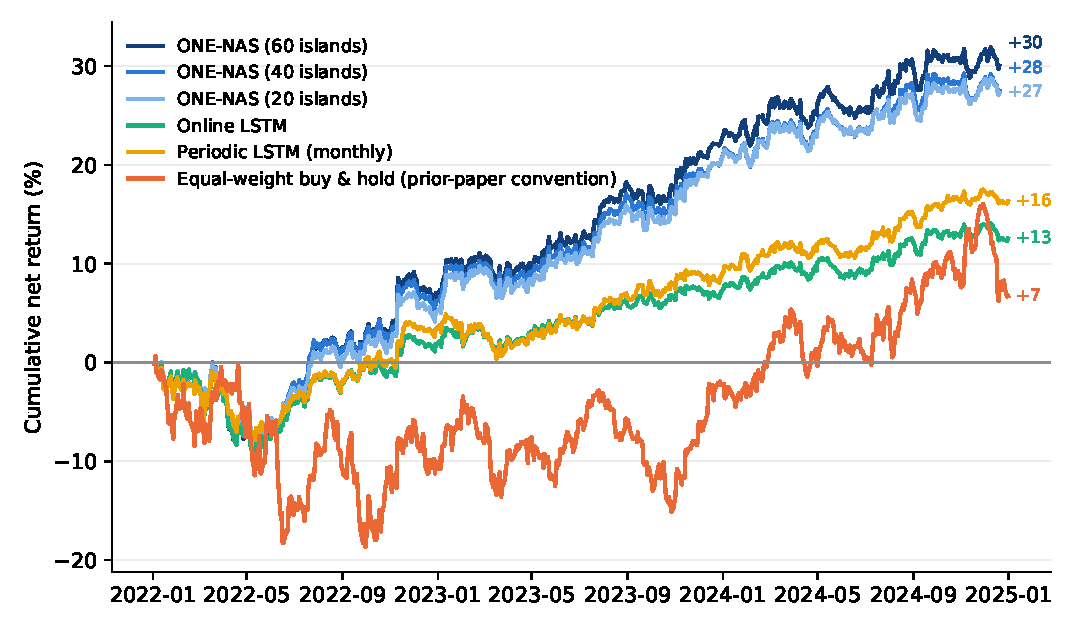
\includegraphics[width=0.92\textwidth]{net_curves.pdf}
\caption{Cumulative net return, 2022--2024 (books restarted at window
start). Buy-and-hold follows the prior-study benchmark convention.}
\label{fig:curves}
\end{figure*}

The more informative comparison is inside the system rather than against
the baselines. The single global-best genome --- the prediction rule of
prior ONE-NAS work --- returns $+4.5\%$ at 40 islands, $+4.7\%$ at 20 and
$+1.0\%$ at 60 (Table~\ref{tab:window}). Those figures sit below every
neural baseline and below buy and hold. The same runs, read as an
ensemble of island champions rather than as a single champion, return
$+27.5$, $+27.4$ and $+30.1$. The search therefore does not pay by
finding one good architecture; it pays by producing a population.


\begin{table}[t]
\centering
\footnotesize
\begin{tabular}{@{}lrr@{}}
\toprule
Comparison & $\Delta$net & paired $t$ \\
\midrule
vs.\ ONE-NAS (60 isl.)       & $-2.5$  & $-1.63$ \\
vs.\ ONE-NAS (20 isl.)       & $+0.2$  & $0.10$ \\
vs.\ Online LSTM             & $+16.2$ & $7.32$ \\
vs.\ Online GRU              & $+15.8$ & $6.59$ \\
vs.\ Periodic LSTM (monthly) & $+12.7$ & $6.66$ \\
vs.\ Online AR$^{a}$         & $+34.9$ & $2.22$ \\
\bottomrule
\end{tabular}
\par\smallskip
{\footnotesize
Comparisons are over all 40 (panel, seed) cells unless noted. Buy \& hold
trades once and is not seed-paired, so no paired test is reported against
it. $^{a}$Deterministic; one run per panel, so $n{=}4$.\par}
\caption{Paired significance for Table~\ref{tab:window}: within-cell
difference in net return (\%) between ONE-NAS (40 islands, sleeves book)
and each other arm, over the (panel, seed) cells the two arms share,
2022--2024.}
\label{tab:paired}
\end{table}

\begin{table}[t]
\centering
\footnotesize
\begin{tabular}{@{}l@{\hspace{3pt}}r@{\hspace{3pt}}r@{\hspace{3pt}}r@{\hspace{3pt}}r@{\hspace{3pt}}r@{}}
\toprule
Arm & $1\times$ & $2\times$ & $3\times$ & $5\times$ & B/E$^{a}$ \\
\midrule
ONE-NAS (60 isl.)   & $+30.1$ & $+27.2$ & $+24.4$ & $+18.8$ & $11.6\times$ \\
ONE-NAS (40 isl.)   & $+27.5$ & $+24.7$ & $+21.8$ & $+16.0$ & $10.6\times$ \\
ONE-NAS (20 isl.)   & $+27.4$ & $+24.4$ & $+21.5$ & $+15.6$ & $10.3\times$ \\
Periodic LSTM       & $+14.8$ & $+11.4$ & $+8.0$  & $+1.2$  & $5.4\times$ \\
Online GRU          & $+11.7$ & $+8.3$  & $+4.9$  & $-1.8$  & $4.5\times$ \\
Online LSTM         & $+11.3$ & $+8.1$  & $+4.9$  & $-1.5$  & $4.5\times$ \\
Online AR           & $-3.3$  & $-6.0$  & $-8.8$  & $-14.2$ & --- \\
\bottomrule
\end{tabular}
\par\smallskip
{\footnotesize
Scaling multiplies the realised per-name cost, so the cross-sectional
shape of costs is preserved and wide-spread names remain the expensive
ones. The $1\times$ column is the sleeves-book column of
Table~\ref{tab:window}. $^{a}$Break-even: the cost multiple at which net
return reaches zero.\par}
\caption{Cost sensitivity: net return (\%) on 2022--2024 as the realised
per-name transaction cost is scaled by the stated multiple. ONE-NAS
tolerates the harshest cost assumption of any arm.}
\label{tab:costs}
\end{table}

Nor do the results depend on an optimistic cost assumption.
Table~\ref{tab:costs} scales the realised per-name transaction cost while
preserving its cross-sectional shape. The ensemble remains profitable to
roughly $10$--$12\times$ realistic costs, against $4.5$--$5.4\times$ for
the baselines. Part of that margin is lower trading: the ensemble turns
over about $0.12$ of gross book per day against $0.13$--$0.14$ for the
baselines, so it pays the scaled cost on less notional.


\begin{table*}[t]
\centering
\small
\begin{tabular}{@{}llrrrr@{}}
\toprule
Fleet & Window & Single & Ensemble & $\Delta$net ($t$) & $\Delta$Sharpe ($t$) \\
\midrule
60 isl.\ ($n{=}10$) & 2022--24 & $+1.0$ / $0.09$  & $+30.1$ / $0.93$ & $+29.1$ $(18.3)$ & $+0.84$ $(14.1)$ \\
40 isl.\ ($n{=}10$) & 2022--24 & $+4.5$ / $0.21$  & $+27.5$ / $0.87$ & $+23.0$ $(18.2)$ & $+0.66$ $(14.7)$ \\
20 isl.\ ($n{=}10$) & 2022--24 & $+4.7$ / $0.25$  & $+27.4$ / $0.87$ & $+22.6$ $(14.9)$ & $+0.62$ $(14.9)$ \\
\midrule
40 isl.\ ($n{=}5$)$^{a}$ & 2016--19 & $+8.9$ / $0.30$  & $+36.7$ / $1.22$ & $+27.8$ $(7.5)$  & $+0.92$ $(6.6)$ \\
\bottomrule
\end{tabular}
\par\smallskip
{\footnotesize $^{a}$Replication on the 2016--2019 tuning-span fleets.\par}
\caption{Prediction rule, within-run paired: single global-best genome
vs.\ island-champion rank-mean ensemble from the same runs (sleeves book).
Net \% / Sharpe; $\Delta$ = ensemble $-$ single, paired $t$ over seeds.}
\label{tab:m1}
\end{table*}

Table~\ref{tab:m1} makes the comparison within-run and paired, since both
rules are scoring-time readings of the same evolved population: the
ensemble adds $+23.0$ points at 40 islands ($t=18.2$), $+22.6$ at 20
($t=14.9$) and $+29.1$ at 60 ($t=18.3$), with Sharpe gains of $+0.62$ to
$+0.84$ on the same pairing. Nothing about the search changes between the
two columns --- only which genomes are read.


\begin{figure}[t]
\centering
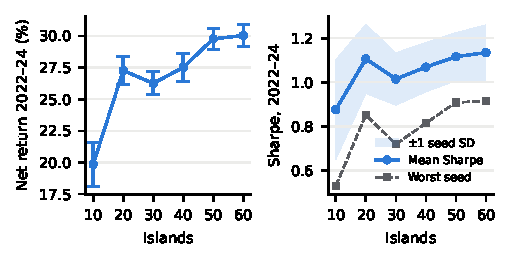
\includegraphics[width=\columnwidth]{islands_scaling.pdf}
\caption{Performance vs.\ island count (2022--2024, registered sleeves
book; 10 seeds $\times$ 4 panels at every width). Left: pooled net return
(mean $\pm$ SE). Right: Sharpe --- mean with $\pm$1 seed-SD band, and the
worst seed. Both rise steeply from 10 to about 20 islands ($+19.9 \to
+27.3$ net, Sharpe $0.88 \to 1.11$) and then flatten: across 20--60 the
cells span $+26$ to $+30$ net and Sharpe $1.01$--$1.13$, and are not
separable at this replication. Seed dispersion narrows over the same
range (SD $0.227 \to 0.11$--$0.13$; worst seed $0.53 \to 0.91$), so the
widest settings are the most reliable as well as the strongest, though
the improvement is not monotone width by width. The 40-island headline
was fixed on the 2016--2019 tuning span (Table~\ref{tab:tunewidth})
before this curve was measured, and the nominally higher 50- and
60-island cells are evaluation-span measurements that were tested on the
tuning span and found indistinguishable from 40.}
\label{fig:islands}
\end{figure}

\begin{table}[t]
\centering
\footnotesize
\begin{tabular}{@{}r@{\hspace{5pt}}r@{\hspace{5pt}}r@{\hspace{5pt}}r@{\hspace{5pt}}r@{\hspace{5pt}}r@{}}
\toprule
Islands & $n$ & rank IC & Net\% & Sharpe & MDD\% \\
\midrule
8  & 20 & $+0.0132$ & $+26.0$ & $0.92$ & $11.6$ \\
16 & 20 & $+0.0149$ & $+31.5$ & $1.11$ & $10.2$ \\
20 & 20 & $+0.0157$ & $+36.0$ & $1.24$ & $10.4$ \\
40 & 40 & $+0.0169$ & $+36.2$ & $1.21$ & $10.4$ \\
50 & 40 & $+0.0170$ & $+36.4$ & $1.21$ & $10.4$ \\
60 & 40 & $+0.0168$ & $+35.7$ & $1.19$ & $10.8$ \\
\bottomrule
\end{tabular}
\par\smallskip
{\footnotesize
$n$ is (panel, seed) cells; widths 8--20 were run at seeds 42--46 and
40--60 at 42--51. Restricting every width to the shared seeds 42--46
leaves the ordering unchanged.\par}
\caption{Island count on the tuning span, 2016--2019, registered sleeves
book. This is the span on which the width was chosen. Rank IC rises from
8 to about 20 islands and is flat above it: the 40-, 50- and 60-island
cells span $0.0168$--$0.0170$ and are not separable (paired against 40,
largest $|t|=0.23$). The 40-island headline therefore sits on the
plateau, while the 8-island setting of the original registration is
measurably below it.}
\label{tab:tunewidth}
\end{table}

Figure~\ref{fig:islands} separates two things that island count does.
Return and Sharpe rise steeply from 10 to about 20 islands ($+19.9$ to
$+27.3$ net, Sharpe $0.88$ to $1.11$) and then flatten: across 20 to 60
the pooled net sits between $+26$ and $+30$ and the widths are not
separable at ten seeds. Seed dispersion narrows over the same range, the
standard deviation of per-seed Sharpe falling from $0.227$ at 10 islands
to $0.11$--$0.13$ above 30 and the worst seed rising from $0.53$ to
$0.91$, though not monotonically width by width. Width therefore buys
consistency at least as much as expected return, which is the relevant
property for a deployed system, where a single run is held rather than an
average over runs.

Width was chosen on the tuning span, not on this curve.
Table~\ref{tab:tunewidth} gives the same sweep on 2016--2019: rank IC
rises from 8 to about 20 islands and is flat above it, with the 40-, 50-
and 60-island cells spanning $0.0168$--$0.0170$. Measured on the trading
period 50 and 60 islands score above 40; measured on the tuning span,
where a configuration choice can legitimately be made, they are
indistinguishable from it (largest $|t|=0.23$). The apparent width
advantage does not survive protocol-symmetric selection and is not
adopted.


\begin{table}[t]
\centering
\footnotesize
\begin{tabular}{@{}l@{\hspace{4pt}}r@{\hspace{4pt}}r@{\hspace{4pt}}r@{\hspace{4pt}}r@{}}
\toprule
Arm & bps/day & \%/yr & NW $t$ & Beta \\
\midrule
ONE-NAS (60 islands)     & $+4.43$ & $+11.2$ & $+2.73$ & $+0.120$ \\
ONE-NAS (40 islands)     & $+4.05$ & $+10.2$ & $+2.56$ & $+0.109$ \\
ONE-NAS (20 islands)     & $+3.99$ & $+10.0$ & $+2.77$ & $+0.114$ \\
Periodic LSTM (monthly)  & $+2.39$ & $+6.0$  & $+2.01$ & $+0.046$ \\
Online LSTM              & $+1.93$ & $+4.9$  & $+1.61$ & $+0.069$ \\
Online GRU               & $+1.75$ & $+4.4$  & $+1.91$ & $+0.033$ \\
Online AR                & $-0.81$ & $-2.1$  & $-0.64$ & $+0.045$ \\
\midrule
Buy \& hold              & $-0.91$ & $-2.3$  & $-0.72$ & $+0.802$ \\
\bottomrule
\end{tabular}
\caption{Factor-adjusted alphas: pooled daily book returns regressed on
the Fama--French three factors plus momentum, 2022--2024, Newey--West lag
10. All three ONE-NAS widths clear $|t|{>}2$; among the baselines only the
monthly-retrained LSTM does, at $t{=}2.01$.}
\label{tab:alphas}
\end{table}

The returns are not explained by factor exposure. Regressed on the
Fama--French three factors plus momentum with Newey--West standard errors
(Table~\ref{tab:alphas}), all three ONE-NAS widths carry alphas
distinguishable from zero ($+10.0$ to $+11.2\%$/yr, $t=2.56$ to $2.77$)
at market betas near $0.11$--$0.12$. Among the baselines only the
monthly-retrained LSTM reaches $|t|=2$, at $+6.0\%$/yr and $t=2.01$;
buy and hold earns no alpha at all ($-2.3\%$/yr, $t=-0.72$) at a market
beta of $0.80$.


\begin{table}[t]
\centering
\footnotesize
\begin{tabular}{@{}l@{\hspace{3pt}}c@{\hspace{3pt}}c@{\hspace{3pt}}c@{\hspace{3pt}}c@{\hspace{3pt}}c@{}}
\toprule
Fleet & $N$ & $\rho$ & Member & Ensemble & Predicted \\
\midrule
20 islands & 20 & 0.166 & $+0.0068$ & $+0.0145$ & $+0.0149$ \\
40 islands & 40 & 0.150 & $+0.0065$ & $+0.0153$ & $+0.0156$ \\
60 islands & 60 & 0.163 & $+0.0067$ & $+0.0157$ & $+0.0160$ \\
\bottomrule
\end{tabular}
\caption{Ensemble diversity mechanism: member rank IC, pairwise member
prediction correlation $\rho$, measured ensemble IC, and the
equicorrelated averaging prediction $m\sqrt{N/(1+(N-1)\rho)}$.}
\label{tab:diversity}
\end{table}

The size of that gain is not an empirical surprise once member diversity
is measured. Table~\ref{tab:diversity} reports, for each width, the mean
rank IC of an individual island champion, the mean pairwise Spearman
correlation $\rho$ between member cross-sections, and the resulting
ensemble IC. Members are individually weak (rank IC $+0.0065$ to
$+0.0068$) and substantially decorrelated ($\rho$ between $0.150$ and
$0.166$). The equicorrelated averaging prediction
$m\sqrt{N/(1+(N-1)\rho)}$ then anticipates the measured ensemble IC to
within 3\% at every width. The ensemble is not recovering a latent
strong model; it is averaging many weak, weakly-correlated ones, and the
observed gain is the size that diversity implies.


\begin{table}[t]
\centering
\small
\begin{tabular}{@{}lr@{\quad}lr@{}}
\toprule
Configuration & $\Delta$net & Configuration & $\Delta$net \\
\midrule
C0 (registered)      & $+3.9$  & NTS 600            & $+12.8$ \\
Select: IC-gated     & $+0.5$  & Rounds 2           & $+11.0$ \\
Select: IC           & $+2.8$  & PER $\alpha$ 0.4   & $+4.0$  \\
Target: 5-day CS     & $+4.5$  & PER $\alpha$ 0.8   & $+11.7$ \\
5-day CS + IC-gated  & $+1.8$  & PER $\lambda{\times}3$ & $+20.6$ \\
Elite 5 / gen 10     & $+9.6$  & BP epochs 20       & $+12.5$ \\
Elite 5 / gen 15     & $+11.1$ & Repop.\ 25         & $+7.0$  \\
Repop.\ 100          & $+9.6$  & PER off (uniform)  & $+9.3$  \\
\bottomrule
\end{tabular}
\par\smallskip
{\footnotesize Mean $+8.3$; $n{=}6$ runs per cell (2 panels $\times$ 3
seeds).\par}
\caption{Ensembling gain (ensemble $-$ single champion, within-run, net \%
on 2016--2019) inside every trained hyperparameter configuration; positive
in 16/16 cells.}
\label{tab:invariance}
\end{table}

The effect does not depend on the configuration it was measured in.
Table~\ref{tab:invariance} recomputes the ensemble-minus-champion
difference inside all 16 trained hyperparameter configurations of the
screen --- different selection metrics, target horizons, population
ratios, repopulation frequencies, replay settings and training budgets.
The difference is positive in 16 of 16, with a mean of $+8.3$ points.
It also holds at every island width tested on the trading period, and at
40 islands on the tuning span as well (Table~\ref{tab:m1}).


\begin{table}[t]
\centering
\small
\begin{tabular}{@{}lr@{}}
\toprule
Population evolving online since 2020-01 & $+26.5$ \\
Cold start at 2022-01                     & $+12.3$ \\
\bottomrule
\end{tabular}
\caption{Online continuity: pooled net (\%) on 2022--2024, frozen 8-island
configuration.}
\label{tab:continuity}
\end{table}

\begin{table}[t]
\centering
\footnotesize
\begin{tabular}{@{}l@{\hspace{4pt}}l@{}}
\toprule
Hyperparameter & Value \\
\midrule
Islands & 40 (headline); 8 (reg.) \\
Elite population / island & 8 \\
Generated / island / generation & 5 \\
Repopulation frequency & every 50 gen. \\
Selection metric & validation MSE \\
Prediction rule & champion rank-mean \\
Target & 1-day CS rank-normal \\
Seq.\ len.\ / step / val.\ sets & 40 / 5 / 5 \\
Train subseq.\ / genome & 2000 \\
Backprop.\ epochs / genome & 10 \\
Replay (PER) $\alpha$, $\lambda$, $\epsilon$ & 0.6, 0.007, $10^{-8}$ \\
Rounds / generation & 1 \\
Node types & simple, UGRNN, MGU, \\
 & GRU, $\Delta$-RNN, LSTM \\
Mut.\ / intra- / inter-crossover & 0.7 / 0.2 / 0.1 \\
Warm-up generations & 50 \\
\bottomrule
\end{tabular}
\caption{ONE-NAS hyperparameter settings (selected on 2016--2019
validation data, disjoint from the evaluation span). Replay sampling
ablated: PER vs.\ uniform shows no advantage on the tuning objective
($\Delta$IC $-0.0024$, $t{=}-1.9$).}
\label{tab:hps}
\end{table}

Three limits are worth stating with the results.

The comparison against buy and hold is not like for like. The ensemble
returns $+27.5\%$ against $+7.9\%$ for an equal-weight hold of the same
universe, but the two carry very different risk: the hold runs at a
market beta of $0.80$ and earns no alpha once factors are accounted for
($-2.3\%$/yr, $t=-0.72$), while the ensemble runs near $0.11$. The
benchmark is included because the prior study on these panels reported
it, and it should be read as a market reference rather than as a
competing strategy.

Second, the evidence is from one universe and one asset class.
Mid-capitalisation US equities over three years is a single regime
sample, and the panels have fixed membership, so the universe is
conditioned on names that survived to the end of it. That conditioning
applies equally to every arm compared here, but it does mean the absolute
return levels should not be read as achievable ex ante.

Third, the prediction rule that pays is also the expensive one to serve.
The ensemble requires every island champion to be evaluated at inference,
so a deployment carries $N$ networks rather than one. The cost is modest
for the small recurrent networks the search produces --- and
Table~\ref{tab:costs} shows the resulting book tolerates transaction
costs far beyond realistic levels --- but it is a real difference from
serving the single champion, and it grows with the island count that
Figure~\ref{fig:islands} recommends.
